\chapter{Analyse}
In dit onderzoek gaat er onderzocht worden of het S88 protocol nagebouwd kan worden met een XILINX Spartan 3E FPGA bord en de harware omschrijf taal VHDL.
\section{deelvragen}
Voor de Analyse zijn er meerdere deelvragen opgesteld,

\begin{enumerate}
	\item Hoe werkt het s88 protocol?
	\item Hoe werkt een XILINX Spartan 3E FPGA bord?
	\item Hoe kan de hardware beschrijving taal VHDL gebruikt worden op het XILINX bord?
	\item Hoe kan een schuifregister aangesloten worden op het XILINX bord?
\end{enumerate}

\subsection{Hoe werkt het s88 protocol?}
Het s88 wordt uitgelegd met behulp van onderstaande afbeelding.
\\\\
Hierin is CENTRALE het in dit project gebruikte XILINX bord. 
\\\\
Een centrale, die hier CENTRALE heet, kan met behulp van het s88 protocol de rechter bus uitlezen. Dit gebeurt met behulp van een schuifregister.
\\\\
Met de DATA OUT poort van de CENTRALE BUS wordt data ingelezen. Deze is verbonden met de Q1 out poort van het schuifregister, hiermee wordt dus informatie van het schuifregister naar de CENTRALE overgedragen.
\\\\
De werking is als volgt, op het moment dat de CENTRALE een positieve flank geeft op de CLOCK en de LATCH hoog is, dan zal het schuifregister de data op Ingang D inlezen. Geeft de CENTRALE een positieve flank en is de LATCH Laag, dan zal het schuifregister één positie opschuiven.
\\\\
Door een puls op RESET te geven worden de buffers gereset en zijn deze weer gereed voor het ontvangen van nieuwe data. 


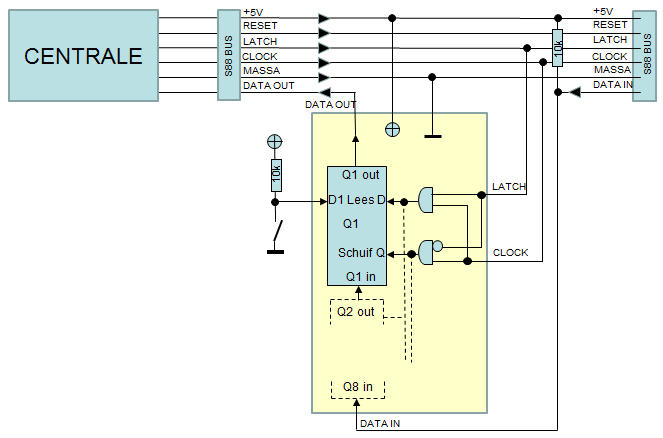
\includegraphics[width=400px]{./img/S88Bus.png}
%http://users.telenet.be/RedDeBist/MBAAN/S88%20terugmelder.htm#S88 bus:
@online{ID,\\
	title = {S88 TERUGMELDERS},\\
	date = {04-03-2016},\\
	url = \url{http://users.telenet.be/RedDeBist/MBAAN/S88\%20terugmelder.htm}
		
	}
\clearpage
	
\subsection{Hoe wordt het XILINX Spartan 3E FPGA bord gebruikt?}
%http://www.xilinx.com/support/documentation/data_sheets/ds312.pdf
Het FPGA bord krijgt instructies in de Hardware programeer taal VHDL om via het S88 protocol te controleren of er iets gebeurd op het RM88 bord. Dit houd in dat het FPGA bord een 'Clock' nodig heeft om te reageren op inkomende 'data' van het RM88 bord.\\
Dit wordt tot stand gebracht door op het FPGA bord via GPIO poorten verbinding te leggen naar het eerder vernoemde RM88 bord. To be continued